
\section{Results}

\begin{frame}[fragile]{Results CIFAR 10 - CIFAR 100}
  \framesubtitle{Tiny Model has some strength in him}
  TinyViT outperforms CNNs on both datasets. Handles complex class distributions better than CNNs.
  \begin{columns}
    \begin{column}{0.7\textwidth}
      \begin{table}[h!]
        \centering
        \sisetup{table-format=2.2}
        \begin{tabular}{@{} l l *{5}{S} @{}}
          \toprule
          \textbf{Dataset} & \textbf{Model} & \textbf{Accuracy} & \textbf{F1} & \textbf{Recall} & \textbf{MCC} & \textbf{Precision} \\
          \midrule

          \multirow{2}{*}{CIFAR-10}
          & \textbf{Tiny ViT} & \textbf{82.59} & \textbf{82.43} & \textbf{82.59} & \textbf{80.70} & \textbf{82.76} \\
          & CNN & 80.67 & 80.55 & 80.67 & 78.53 & 80.56 \\

          \multirow{2}{*}{CIFAR-100}
          & \textbf{Tiny ViT} & \textbf{59.40} & \textbf{59.04} & \textbf{59.40} & \textbf{59.00} & \textbf{60.00} \\
          & CNN      & 46.13 & 44.57 & 46.13 & 45.61 & 45.61 \\
          \bottomrule
        \end{tabular}
        \vspace{0.2cm}
        \small Note: All values are percentages (\%). Bold indicates best performance in category.
      \end{table}
    \end{column}
  \end{columns}
\end{frame}

\begin{frame}[fragile]{Results STL-10}
  \framesubtitle{CNNs outperforms our Tiny Model}
  CNN performs better on STL-10, likely due to the higher image resolution. TinyViT may struggle with lower-resolution images in datasets with fewer samples.
  \begin{columns}
    \begin{column}{0.7\textwidth}
      \begin{table}[h!]
        \centering
        \sisetup{table-format=2.2}
        \begin{tabular}{@{} l l *{5}{S} @{}}
          \toprule
          \textbf{Dataset} & \textbf{Model} & \textbf{Accuracy} & \textbf{F1} & \textbf{Recall} & \textbf{MCC} & \textbf{Precision} \\
          \midrule
          \multirow{2}{*}{STL-10}
          & Tiny ViT & 64.27 & 64.30 & 64.27 & 60.47 & 66.13 \\
          & \textbf{CNN}      & \textbf{68.36} & \textbf{68.10} & \textbf{68.36} & \textbf{64.95} & \textbf{68.78} \\
          \bottomrule
        \end{tabular}
        \vspace{0.2cm}
        \small Note: All values are percentages (\%). Bold indicates best performance in category.
      \end{table}
    \end{column}
  \end{columns}
\end{frame}

\begin{frame}[fragile]{Confusion Matrices}
  \framesubtitle{Visualize the results}
  \begin{columns}
    \begin{column}{0.3\textwidth}
      \begin{figure}[!ht]
        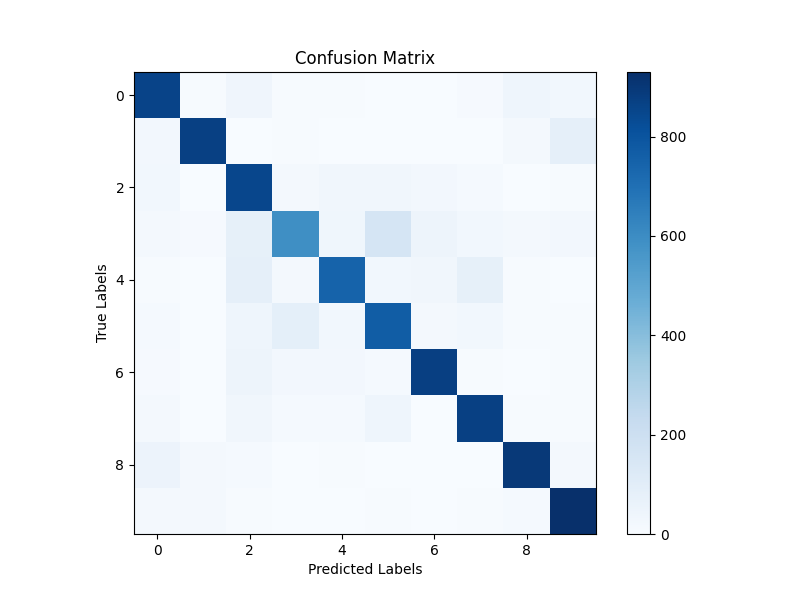
\includegraphics[width=\textwidth]{images/cifar10_cm.png}
        \small CIFAR-10 dataset using Tiny ViT
      \end{figure}
    \end{column}

    \begin{column}{0.3\textwidth}
      \begin{figure}[!ht]
        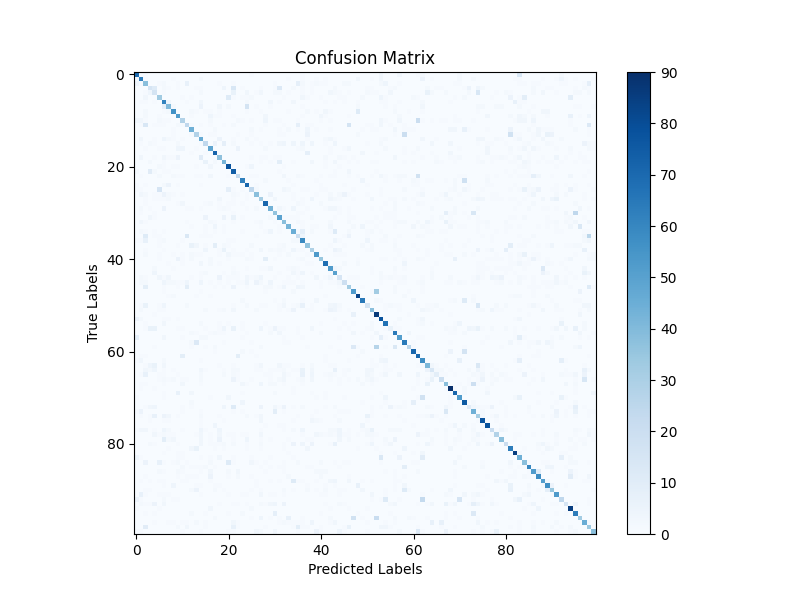
\includegraphics[width=\textwidth]{images/cifar100_cm.png}
        \small CIFAR-100 dataset using Tiny ViT
      \end{figure}
    \end{column}

    \begin{column}{0.3\textwidth}
      \begin{figure}[!ht]
        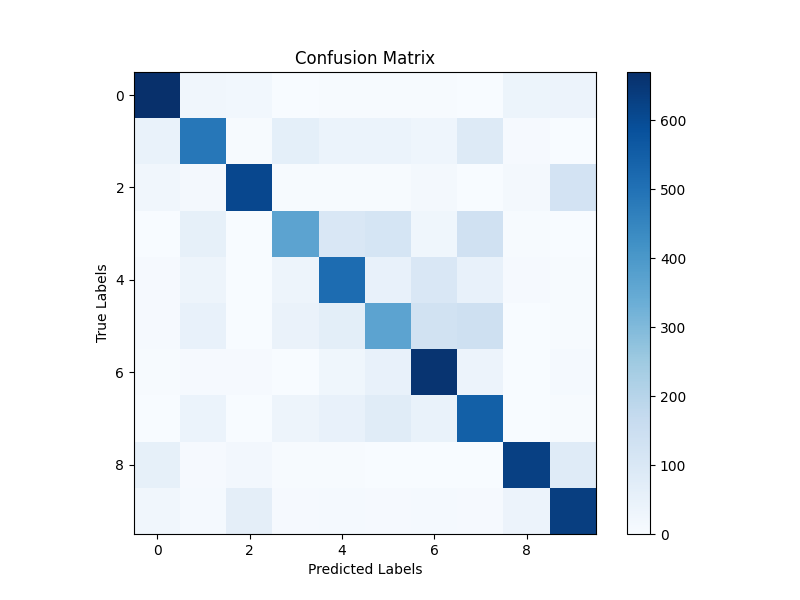
\includegraphics[width=\textwidth]{images/stl10_cm.png}
        \small STL-10 dataset using CNN
      \end{figure}
    \end{column}
  \end{columns}
\end{frame}